\documentclass[10pt]{article}
\usepackage[margin=1in]{geometry}
\usepackage{amsmath, amssymb, bm, mathtools}
\usepackage{graphicx, subfig, wrapfig, mwe, epstopdf, pdfpages}
\usepackage{listings}
%\usepackage[section]{placeins}
\usepackage{enumerate}
\usepackage{stmaryrd}
\usepackage{algorithm, algpseudocode}
\usepackage{float}
\usepackage[hidelinks]{hyperref}
\usepackage{url}
\usepackage[toc, nonumberlist]{glossaries}
\newglossary{symbol}{sym}{sbl}{List of Discretization Symbols}
\include{glossary}

% set paragraph indentation to be 0 by default
\setlength\parindent{0pt}

% macros
\newcommand{\bigO}[1]{\mathcal{O}\left(#1\right)}
\newcommand{\LL}[1]{L^{2}\left(#1\right)}
\newcommand{\LLW}{\LL{\Omega}}
\newcommand{\Hdiv}[1]{H^{\text{div}}\left(#1\right)}
\newcommand{\HdivW}{\Hdiv{\Omega}}
\newcommand{\Th}{\mathcal{T}_h}
\newcommand{\dTh}{\partial\mathcal{T}_h}
\newcommand{\uhath}{\widehat{u}_h}
\newcommand{\qhath}{\widehat{\bm{q}}_h}
\newcommand{\lims}[2]{\bigg\rvert^{#1}_{#2}}
\newcommand{\at}[1]{\lims{}{#1}}

\newcommand{\LLN}[1]{\left\Vert #1 \right\Vert_{\LLW}}
\newcommand{\HN}[1]{\left\Vert #1 \right\Vert_{H^1(\Omega)}}
\newcommand{\HSN}[1]{\left| #1 \right|_{H^1(\Omega)}}
\newcommand{\Hb}{H^{1,\text{broken}}}
\newcommand{\HbW}{H^{1,\text{broken}}(\Omega)}

% DG integrals, jumps 
\newcommand{\Iint}[3]{\left(#1 ,\, #2 \right)_{#3}}
\newcommand{\IintK}[2]{\Iint{#1}{#2}{K}}
\newcommand{\Eint}[3]{\left\langle #1 ,\, #2 \right\rangle_{#3}}
\newcommand{\EintK}[2]{\Eint{#1}{#2}{\partial K}}
\newcommand{\jmp}[1]{\llbracket #1 \rrbracket}

% physics
\newcommand{\ReL}{\text{Re}_L}
\newcommand{\Pra}{\text{Pr}}
\newcommand{\Pe}{\text{Pe}}

% restriction operator
\newcommand\restr[2]{{ % we make the whole thing an ordinary symbol
  \left.\kern-\nulldelimiterspace % automatically resize the bar with \right
  #1 % the function
  \vphantom{\big|} % pretend it's a little taller at normal size
  \right|_{#2} % this is the delimiter
  }}


\title{Thermal Boundary Layer Energy Equation for Liquid Metal Flow}
\author{Corbin Foucart}
\date{}
\begin{document}
\maketitle

\section{Problem Statement}
We investigate boundary layer heat transfer of fluid flowing over a heated flat plate. The governing
equations are derived in \cite{incropera} as:

\begin{align}
  \frac{\partial u}{\partial x} + \frac{\partial u}{\partial y} &= 0 \\
  u\frac{\partial u}{\partial x} + v\frac{\partial u}{\partial y} 
  &=  -\frac{1}{\rho}\frac{\partial p}{\partial x} + \mu \frac{\partial^2 u}{\partial
  y^2} \\
  u\frac{\partial T}{\partial x} + v\frac{\partial T}{\partial y} 
  &= \frac{k}{\rho c_p} \frac{\partial^2 T}{\partial y^2} + \mu\left[ \frac{\partial u}{\partial
  y}\right]^{2}
  \label{eq:BLeqns}
\end{align}

Where $u,\,v$ are the $x$ and $y$ velocities respectively, $p$ is the pressure, $T$ is the
spatially-varying fluid temperature in the boundary layer, and $\kappa,\, \rho,\, c_p$ are the
thermal conductivity, density, and specific heat of the fluid, respectively. We are interested in
the temperature profile close to the heated plate, and so we make the following assumptions:

\begin{enumerate}
  \item No vertical component of velocity: $v=0$
  \item Specified flow profile: $u(y)$
  \item Neglect viscous dissipation term: $\mu\left[ \frac{\partial u}{\partial y}
    \right]^{2}$ small compared to other terms
\end{enumerate}

Then the governing equation in this regime reduces to:
\begin{align}
  \left[u(y)\right]\frac{\partial T}{\partial x} 
  &= \frac{k}{\rho c_p} \frac{\partial^2 T}{\partial y^2} 
\end{align}

  \subsection{Non-dimensionalization of governing equations}
    Since we don't know what physical parameter values the user is going to provide, we don't want
    to run into scaling issues; therefore we can accept as input the physical parameters, but solve
    a non-dimensionalized version of the problem. \\

    We define $\alpha = \frac{k}{\rho c_p}$, and note the following characteristic problem
    parameters: the characteristic length scale $L$ of the plate, the free-stream velocity
    $U_\infty$,  the heat flux $q$ in [W/m$^2$], and free stream temperature $T_\infty$.
    
    We consider the non-dimensional quantities

      \begin{align}
        x^* \equiv \frac{x}{L} &\qquad y^* \equiv \frac{y}{L} \\
        u^* \equiv \frac{u}{U_\infty} &\qquad T^* \equiv \frac{k(T - T_\infty)}{qL} 
      \end{align}

    where $\Pe = \ReL \Pra = \frac{L U_\infty}{\alpha}$ is the Peclet number. The above
    definitions give rise to the following non-dimensional governing equation

    \begin{align}
      u^*\frac{\partial T^*}{\partial x^*} 
      &=\frac{1}{\Pe}\frac{\partial^2 T^*}{\partial {y^*}^2} 
    \end{align}

    For the boundary conditions, in the case of the plate being heated by a resistance heater or the
    like, we impose a constant flux boundary condition on $\Gamma_1$

    \begin{align}
      \left[k\frac{dT}{dy}\right]_{\Gamma_1} = q
      \qquad \rightarrow \qquad 
      \frac{dT^*}{dy^*}\bigg|_{\Gamma_1} = 1
      \label{eq:fluxBC}
    \end{align}
     
    similarly, the far-field condition at $\Gamma_2$ is that $T = T_\infty \Rightarrow T^* = 0$.
    Having completed the non-dimensionalization of the problem, we are prepared to state the strong
    form.

    \subsection{Strong form}
    We can therefore write the complete strong form
    of the problem as:

    \begin{align}
      u^*\frac{\partial T^*}{\partial x^*} 
      =\frac{1}{\Pe}\frac{\partial^2 T^*}{\partial {y^*}^2} 
      \;\,\text{ on } \Omega=(\Gamma_1,\, \Gamma_2)
    \end{align}

    subject to boundary conditions
    \begin{align}
      \frac{dT^*}{dy^*}\bigg|_{\Gamma_1} = 1,\;
      T^*(x^*,\, \Gamma_2) = 0 \\
      %u^*(x^*, 0) = 0 , u^*(x^*, \infty) = 1
    \end{align}

    Which is the problem which will be discretized and solved numerically. The user will enter as
    inputs to the software $L,\, U_\infty,\, q,\, T_\infty,\, \Pe$. The only concern is that the
    user must enter an $L$ which is large enough to contain the thermal boundary layer.
  
    \subsection{Approximation of $u(y)$ and the computational domain}

    The last piece of the problem statement is the types of velocity profiles to be considered. In
    the physical regime of $\Pr \ll 1$, the thermal boundary layer grows much faster than the
    momentum boundary layer, and we can approximate the velocity field $u^*$ as steady in $x$. We
    consider the two approximations of $u^* = U_\infty$ and a linear profile $u^* = y^*$.

\section{Weak Formulation and Discretization}

    In this section, we drop the non-dimensionalized $^*$ notation for convenience. Note that our
    inhomogenous Dirichlet condition in the dimensional problem reduces to a homogeneous Dirichlet
    condition in the non-dimensional equation. Therefore, our finite element spaces $X^E$ and $X$
    coincide

    \begin{align}
      X^E = X =  \left\{ v \in H^1(\Omega) \mid v(\Gamma_2) = 0 \right\}
    \end{align}

    and we can write our semi-discretized weak form as 

    \begin{align}
      \text{find } w_h(x)\in X^E \text{ such that }
      m\left(u\frac{dw_h}{dx},\, v  \right) + a(w_h,v) = f(v)
    \end{align}

    Where the weak form operators are defined as (see Appendix \ref{app:wkder}):

    \begin{align}
      &m(T,v)  = \int_\Omega u(y) \frac{dT}{dx} v\, dy \\
      &a(T, v) =\frac{1}{\Pe} \int_{\Omega}^{} \frac{dv}{dy} \frac{dT}{dy} \, dy \\
      &f(v)    = \int_{\Omega}^{} f_\Omega v\,dy -\frac{1}{\Pe} v(\Gamma_1)
    \end{align}

    We perform a backward euler discretization in time (since it is unconditionally stable). Then we
    can state our finite element problem for any given $x$ as the following: $\text{find } w_h(x)\in
    X^E \text{ such that }$

    \begin{align}
      m\left(u \frac{w_h^{k+1} - w_h^{k}}{\Delta x},\, v  \right) 
      + a\left(w_h^{k+1},v\right) = f(v)
    \end{align}

    which is equivalent to 

    \begin{align}
      \frac{1}{\Delta x} m\left(u \, w_h^{k+1},\, v  \right) 
      + a\left(w_h^{k+1},v\right) = f(v) - \frac{1}{\Delta x} m(u\, w_h^k,\, v)
    \end{align}

    which completes the problem discretization.  Details on the implementation of the time-stepping
    operators can be found in Appendix \ref{app:m_operator}.

\section{Implementation Details}

  The entire code for the project (numerics, verification, visualization) is written in pure
  \texttt{Python} in the contained iPython notebook \texttt{Project\_1.ipynb}.  For numerical
  integration, we use quadrature rules from the open source library \texttt{quadpy} \cite{quadpy}.
  The notebook additionally contains extended commentary and thorough discussion of implementation
  details, with the intention of walking the reader through the use and development of the code. It
  can be run in part or in its entirety. I have also included a static \texttt{html} file containing
  the output of the notebook run from beginning to end. The following section provides an
  abbreviated summary of notebook sections 4-6 (Verification, Re-dimensionalization, and Physical
  Test Cases). For the details in their entirety, consult either the output or run the notebook
  directly. 

\section{Brief Overview of Results}

  Verification of the code primarily involved test cases using the method of manufactured solutions
  over the non-dimensional computational domain. We provide a temporal convergence study and a
  discussion of variable ``time-stepping''.  The user enters the problem parameters in dimensional
  form; \texttt{Project\_1.ipynb} discusses the implementation of re-dimensionalizing the problem
  and returning the solution on the physical domain, as well as visualization techniques (to which
  we refer the interested reader). Lastly, we consider two physical test cases for low-Prandtl
  liquid metal flows.

  \subsection{Verification}
  \subsubsection{Verification of 1D Implicit FE Solver}

  Before testing the 2D code, it makes sense just to test the 1D implicit spatial solver is working
  correctly.  We test on a small spatial subproblem with strong form

  \begin{align}
    0= \frac{d^2 u}{dx^2} - f_{ex}
  \end{align}

  where we choose $f_{ex}$ as a constant function in space. It doesn't get much simpler than this.
  The general solution is $u = x^2 + bx + c$ and we can symbolically determine the coefficients for
  any choice of boundary conditions $g_N,\, g_D$.  To check that our 1D boundary conditions are
  implemented correctly, we choose an exact solution with inhomogeneous boundary conditions (both
  for Dirichlet and Neumann boundaries).  The results of the manufatured solution test are shown
  below. \\
  
  \centerline{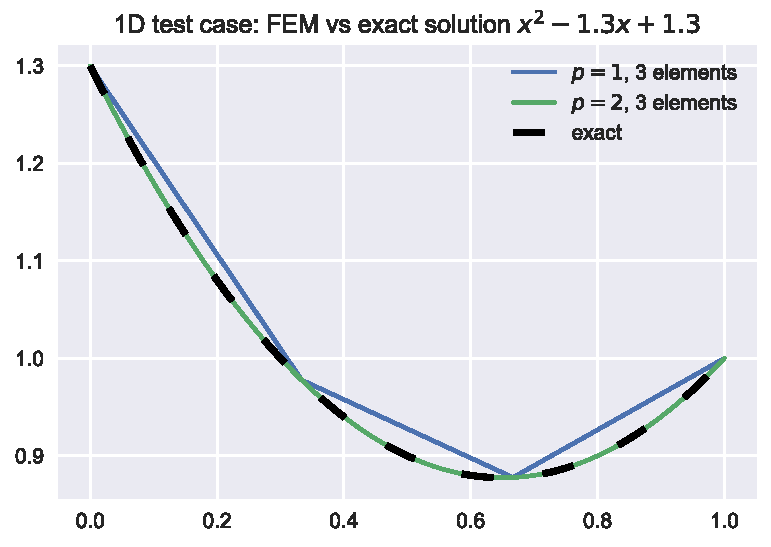
\includegraphics[width=0.65\textwidth]{img/1D_test.pdf}}

  The linear solution looks good and the quadratic solution matches exactly, as we would expect,
  since the exact solution is an element of our finite element approximation space. We could be a
  bit more rigorous about measuring the error here (by choosing an MS outside of a polynomial space
  and measuring error with quadrature), but we consider this overkill for 1D.

  \subsubsection{Verification of 2D ``Temporal'' FE Solver}

  We choose a manufactured solution which satisfies our non-dimensional equation, i.e.,
  some field $w(x, y) = f(x) g(y)$ such that

  \begin{itemize}
    \item $w(x, 1) = g_D$ (dirichlet 0 condition at $y=1$)
    \item $w\frac{d w}{d y}(x, 0) = g_N$ (neumann flux condition)
  \end{itemize}

  For this, we can simply take our exact solution to the 1D test cast and multiply it by some
  $f(x)$, here we choose a decaying exponential $\exp(-3x)$. We then compute the analytical forcing
  function $f_{ex}$ necessary to give us our chosen analytical solution.  

  \begin{align}
    w(x,\, y) &= \left(y^{2} - 1.3 y + 1.3\right) e^{- 3 x} \\
    f_{ex} &=  3 y \left(y^{2} - 1.3 y + 1.3\right) e^{- 3 x} - 2 e^{- 3 x}
  \end{align}
  
  For good measure, we
  choose a velocty profile $u(y) = y$ to test that our quadrature rules are integrating the mass
  operator with the velocity field well. The results of a test at reasonable resolution are below.\\

  \centerline{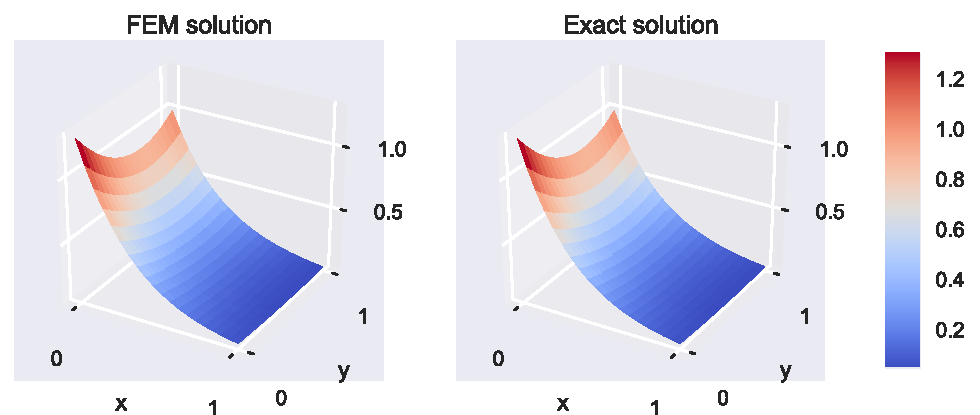
\includegraphics[width=0.85\textwidth]{img/2D_MS_result.pdf}}

  Additionally, we can plot the $L_\infty$ error; computing other error norms is dicey since the
  time and space domains are treated differently -- at least it isn't clear that we can meaningfully
  talk about a finite element solution defined at $x$ points not at $\Delta x$ increments. As we
  expect, the error is close to location corresponding to the beginning of the plate in the
  numerical domain. We also note that our spatial discretization is enormous overkill. Simply taking
  a single $p=2$ element should reproduce the exact solution for each 1D problem, since the solution
  of every spatial problem lies in our $p=2$ finite element space by construction. \\

  \centerline{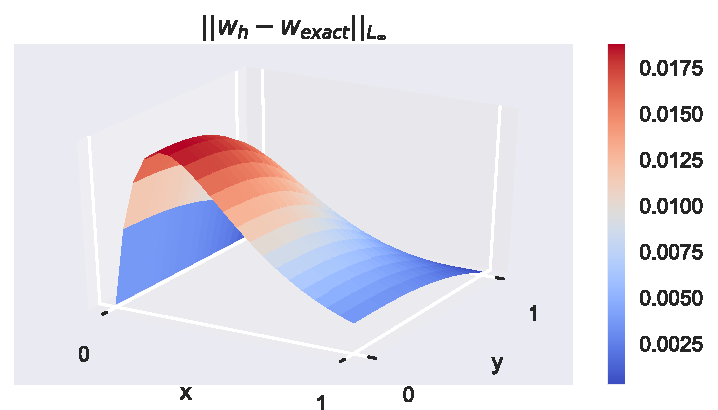
\includegraphics[width=0.45\textwidth]{img/2D_MS_wh-exact.pdf}
  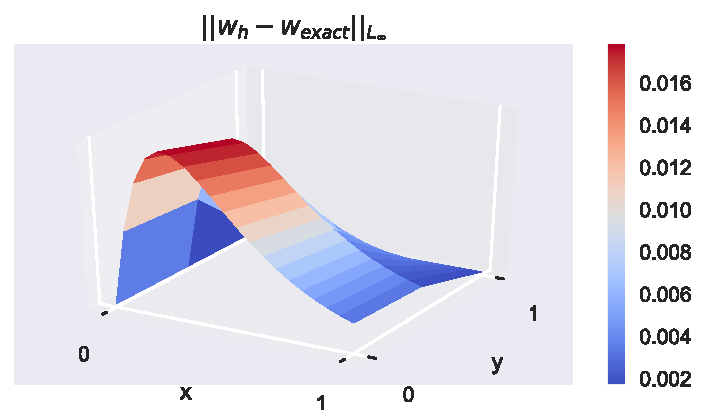
\includegraphics[width=0.45\textwidth]{img/2D_MS_wh-exact_coarse.pdf}}

  Indeed, we see that the $L_\infty$ error is unaffected by coarsening the spatial mesh to a single
  element. It remains to investigate the temporal error.

  \subsubsection{Variable ``Timestepping''}

  Because of the particular features of our problem, we expect numerical issues to occur at the
  leading edge of the heated plate. We would like to investigate the effect of changing the
  computational ``temporal'' domain in $x$ to be more refined closer to the leading edge of the
  plate.  \\

  \centerline{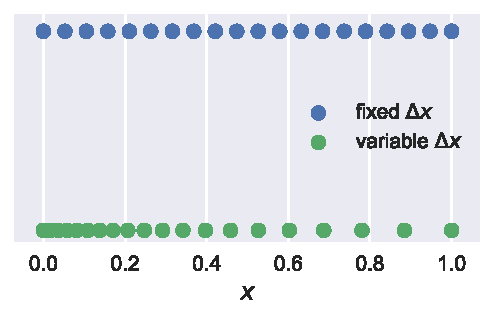
\includegraphics[width=0.5\textwidth]{img/warped_grid.pdf}}

  Above, we see sample output of a warping function which warps the grid according to an exponential
  transform. The code is written sufficiently generally that we can provide a variable timestep. \\

  \subsubsection{Convergence Study}

  Since we have no spatial discretization error, we can measure temporal error to see if we can
  recover order 1 convergence in the $L_\infty$ norm. We can also compare how variable timestepping
  does against regular timesteps. Note that we are running with $p=2$ elements where we know the
  spatial solution is analytically quadratic in order to make sure spatial error is unimportant.

  \centerline{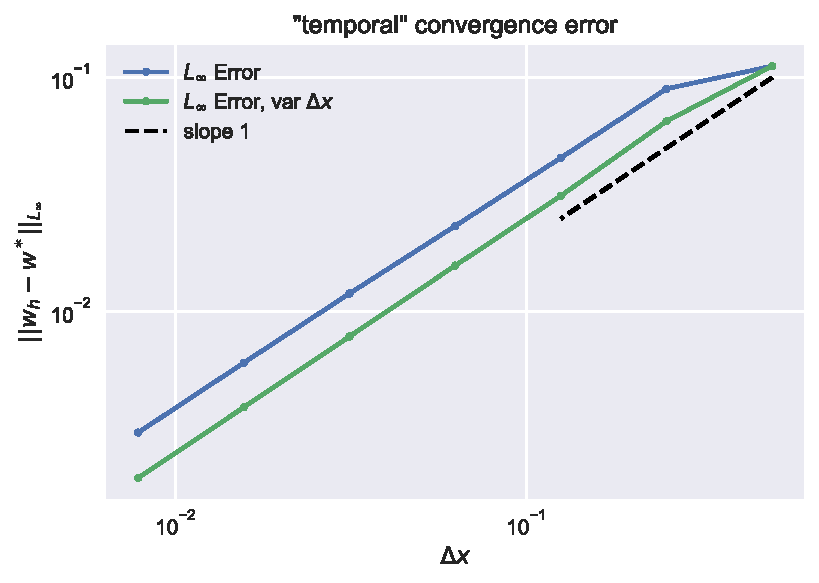
\includegraphics[width=0.65\textwidth]{img/temporal_convergence.pdf}}

  We see that both are converging to first order in time, but that the coefficient on the error is a
  bit lower for the warped grid. As a word of warning, though, we can only get this nice feature
  because we knew where we expected the solution have a steep gradient in time. If we knew nothing
  about our problem, using the variable timestepping in this manner would not help.  It just so
  happens that for our client application, we expect the area of interest to be the start of the
  plate.

  \subsection{Physical Test Cases}

  Now that we are confident that our code is giving the correct solution to the appropriate
  convergence rates for problems slightly more general than our problem of interest, we can consider
  some physical test cases. 

  \subsubsection{Liquid Mercury}
  Test case setup:

  \vspace{0.5cm}
  \begin{lstlisting}[language=Python]
    # liquid mercury -- low Prandtl number
    L     = 1.0      # meter
    U_inf = 5e-2     # m/s
    k     = 8.18     # W / (m deg C)
    q     = -2       # W/m^2
    T_inf = 25       # degrees C
    mu    = 0.16e-2  # N s / m^2
    rho   = 13595    # kg/m^3
    cp    = 0.1404   # J/kgK

    # compute Pr number, make sure it's low
    Pr = cp * mu / k
    ReL = rho * U_inf * L / mu
    Pe = ReL * Pr
  \end{lstlisting}
  \vspace{0.5cm}

  From where we see that $\Pra = 1.75e-5,\, \Pe = 11.7$, in the physical regime in which our
  approximations comfortably hold. We solve the numerical problem on a warped grid, and visualize
  the boundary layer temperature with both height and color. The results can be seen below.\\

  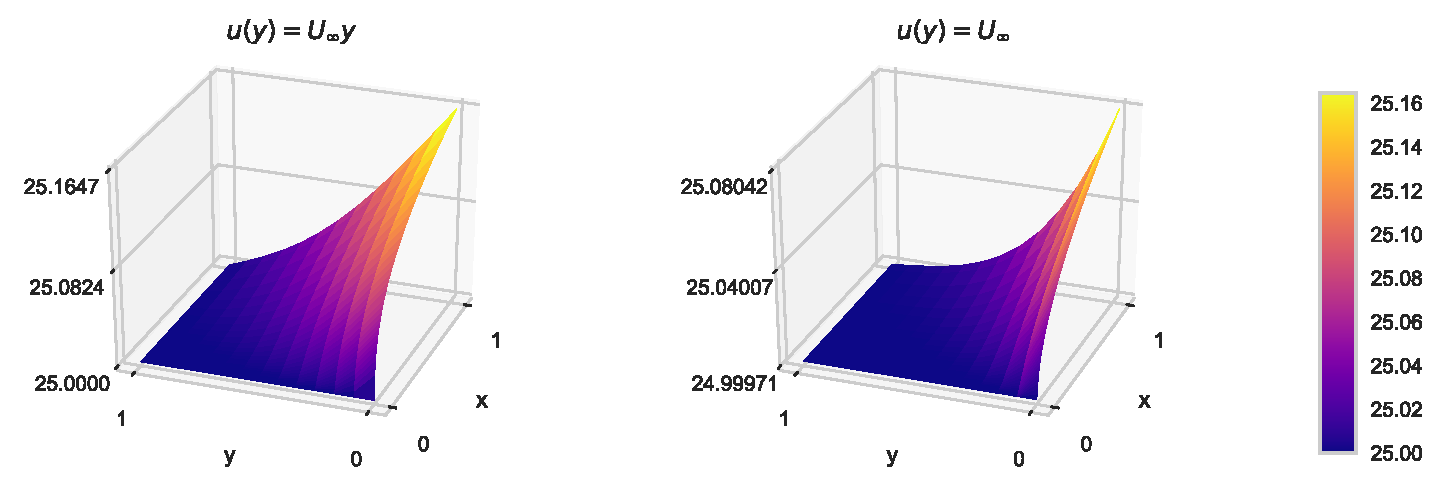
\includegraphics[width=\textwidth]{img/liquid_hg_BL.pdf}
  We can see that when $u = U_\infty$ is constant, the boundary layer growth is slower, as we would
  physically anticipate.

  \subsubsection{Molten Lead}
  Test case setup:

  \vspace{0.5cm}
  \begin{lstlisting}[language=Python]
  # molten lead -- low Prandtl number
  L     = 0.8      # meter
  U_inf = 2e-3     # m/s
  k     = 16.1     # W / (m deg C)
  q     = -20      # W/m^2
  T_inf = 371      # degrees C
  nu    = 2.27e-7  # m^2/s
  alpha = 1.08e-5  # m^2/s
  cp    = 0.159e3  # J/kgK

  # compute Pr number, make sure it's low
  Pr = nu / alpha
  ReL = U_inf * L / nu
  Pe = ReL * Pr
  \end{lstlisting}
  \vspace{1cm}

  Here, $\Pra = 0.021,\, \Pe = 148$, again in the physical regime in which our approximations
  hold, although in this test case, we expect the boundary layer to stay much closer to the edge of
  the computational domain. We solve the problem, once again on the warped grid, and visualize the
  thermal boundary layer with only color (since it is so close to the wall). Further, we
  deliberately use a non-perception neutral colormap \texttt{jet} to accentuate differences in
  temperature.  Results can be seen below. \\

  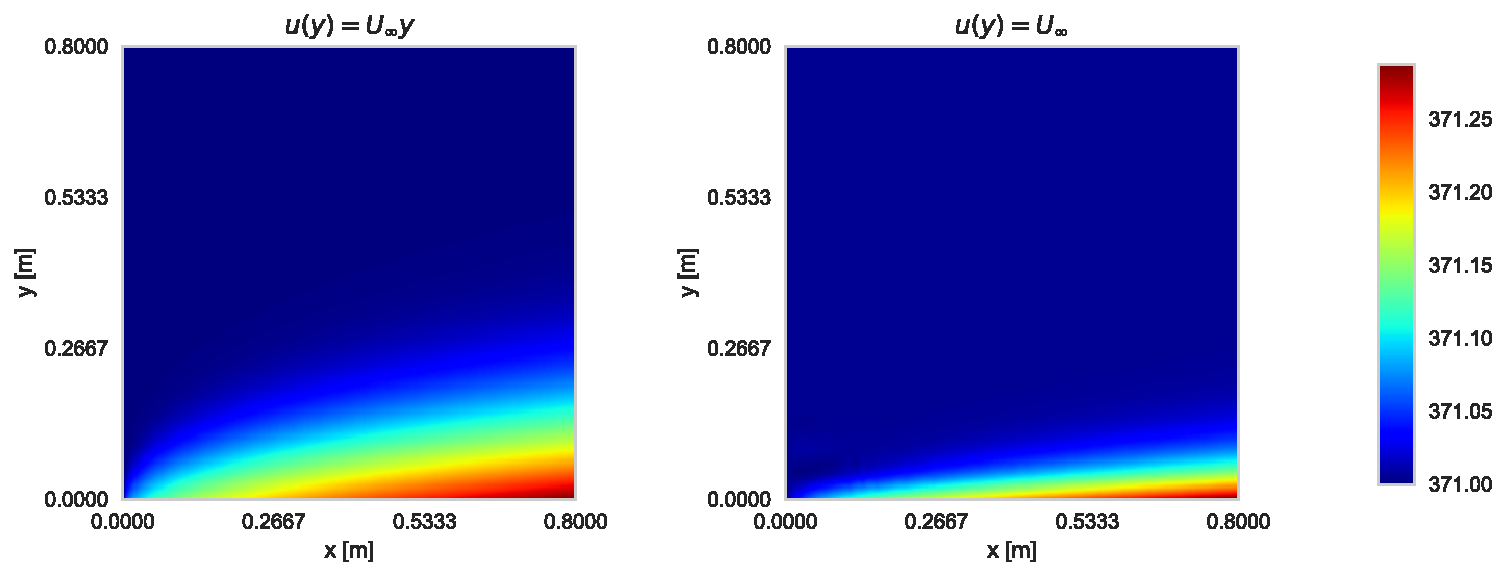
\includegraphics[width=\textwidth]{img/molten_lead_BL.pdf}

  There are some interesting features in this case. Although difficult to see, at the leading edge
  of the heated plate for the $u(y) = U_\infty$ case, the solution has small Gibbs oscillations due to the
  ``free-slip'' constant velocity profile. Note that for the velocity field $u(y) = y$, the velocity
  vanishes at the plate, and the oscillations are not present. In each case, the boundary layer does
  not develop to the extent of the computational domain.

% appendix
\appendix
\section{Weak Form: Derivation} \label{app:wkder}

  We handle the non-dimensional problem, but omit the $^*$ notation for readability. we additionally
  use $\eta$ to denote $x^*$, the pseudo-time variable, and $y$ to denote the spatial coordinate
  $y^*$. We multiply by a test function $v \in X$ and integrate over the spatial domain\footnote{%
    Note that since we are only semi-discretizing, we can write $\frac{d^2 T}{dy^2}$ instead of 
    $\frac{\partial^2 T}{\partial y^2}$. We will complete the discretization of the pseudo-time term
    using finite differences.
  } $\Omega = (\Gamma_1 = 0,\, \Gamma_2)$. \\

  We also consider a slightly more general strong form (we add an arbitrary source term$f_\Omega$)
  so that we can write a general code more easily testable by the method of manufactured solutions;
  namely,

    \begin{align*}
      u \frac{dT}{d\eta} = \frac{1}{\Pe} \frac{d^2T}{dy^2} + f_\Omega
      \;\,\text{ on } \Omega=(\Gamma_1,\, \Gamma_2)
    \end{align*}

  subject to boundary conditions
  \begin{align}
    \frac{dT}{dy}\bigg|_{\Gamma_1} = g_N,\;\;
    T(x,\, \Gamma_2) = g_D \\
    %u^*(x^*, 0) = 0 , u^*(x^*, \infty) = 1
  \end{align}

    \begin{align*}
      \int_\Omega u(y) \frac{dT}{d\eta} v\, dy 
      - \frac{1}{\Pe} \int_{\Omega}^{} \frac{d^2 T}{dy^2} v\, dy 
      &= \int_\Omega u(y) \frac{dT}{d\eta} v\, dy 
      - \frac{1}{\Pe} \int_{\Omega}^{} \left[ \frac{d}{dy}\left( v \frac{dT}{dy} \right) -
      \frac{dv}{dy} \frac{dT}{dy} \right]\, dy \\
      &= \int_\Omega u(y) \frac{dT}{d\eta} v\, dy 
      + \frac{1}{\Pe} \int_{\Omega}^{} \frac{dv}{dy} \frac{dT}{dy} \, dy 
      - \frac{1}{\Pe}\left[ v \frac{dT}{dy} \right]^{\Gamma_2}_{\Gamma_1} \\
      &= \int_\Omega u(y) \frac{dT}{d\eta} v\, dy
      + \frac{1}{\Pe} \int_{\Omega}^{} \frac{dv}{dy} \frac{dT}{dy} \, dy 
      +\frac{1}{\Pe} v(\Gamma_1)
      = \int_{\Omega}^{} f_\Omega v\, dy
    \end{align*}

    where we have applied integration by parts and the divergence theorem. Note that $v(\Gamma_2) =
    0$ by our choice of $X$; note that $\frac{dT}{dy}\big|_{\Gamma_1}=1$ is determined by
    (\ref{eq:fluxBC}). Then we recognize

    \begin{align}
      \underbrace{\int_\Omega u(y) \frac{dT}{d\eta} v\, dy}_{m\left( \frac{dT}{d\eta},\, v \right)}
      + \underbrace{\frac{1}{\Pe} \int_{\Omega}^{} \frac{dv}{dy} \frac{dT}{dy} \, dy }_{a(T, v) }
      = \underbrace{\int_{\Omega}^{} f_\Omega v\,dy -\frac{1}{\Pe} v(\Gamma_1) }_{f(v)}
    \end{align}

    Which completes our derivation of the weak form. 

\section{Quadrature and implementation of $m(\cdot,\, \cdot)$ operator} \label{app:m_operator}
    We briefly remark on the implementation of the $m( \cdot ,\,  \cdot )$ terms.
    For the implicit $m(u\, w_h^{k+1})$, we compute the integral with quadrature, 

    \begin{align}
      \frac{1}{\Delta x}\int_{K_m} u \phi_j \phi_i\, dx 
        = \frac{1}{\Delta x} \int_{\hat{K}} u\widehat{\phi}_i \cdot \widehat{\phi}_j \left| \det
        J\right|\, d\widehat{x}
        \approx
        \frac{1}{\Delta x} \sum_q w_q\, \det J\big|_{x_q}\, u_q(x_q)  \cdot \widehat{\phi}_i(\xi_q) \cdot
        \widehat{\phi}_j(\xi_q) 
      \end{align}
    
    For the explicit term $u\, w_h^k$ is known at time $k+1$, and it can be considered part of the
    body forcing; that is

    \begin{align}
      \frac{1}{\Delta x} m(u\, w_h^k) =
      \int_{\Omega}^{} \underbrace{\frac{u\, w_h^k}{\Delta x}}_{f_{\Delta x}} v \, dx
    \end{align}

    As a final note, we consider the implementation of $f_{\Delta x}$. In order to compute this
    ``forcing'' term with quadrature, we need the values of $w_h^k$ at the physical-space quadrature
    points, whereas they are only computed at the nodal values. However, we can do so efficiently,
    because $w_h^k(x) = \alpha_i \phi_i(x)$, hence for physical space quadrature point $x_q$ and
    corresponding reference element quadrature point $\xi_q$,

    \begin{align}
      w_h^k(x_q) = \alpha_i \phi_i(x_q) 
      = \alpha_i \phi_i(G^{-1}(x_q)) 
      = \alpha_i \phi_i(\xi_q) 
    \end{align}

    where $G,\, G^{-1}$ denote the isoparametric mapping from reference element to physical space and
    the inverse, respectively. Since the values of the shape functions $\phi_i$ are computed on the
    reference element during the problem setup, we can cheaply compute $w_h^k(x_q)$ without needing
    to explicitly compute the inverse transformation $G^{-1}$; caluculate ${S_q}^T \alpha$, where

    \begin{align}
    S_q = 
    \begin{bmatrix}
      \phi_1(\xi_{q_1}),\, &\ldots &\phi_1(\xi_{q_n}) \\
      \vdots && \vdots \\
      \phi_{n_b}(\xi_{q_1}),\,  &\ldots &\phi_{n_b}(\xi_{q_n}) \\
    \end{bmatrix},\, \qquad
    \alpha = \begin{bmatrix} \alpha_1,\, \ldots \alpha_{n_b}\end{bmatrix}
    \end{align}


% bibliography
\nocite{*}
\bibliography{report.bib}{
  \bibliographystyle{plain}}

\end{document}
